\documentclass[17pt, fleqn]{beamer}
\usepackage{default}
\usetheme{default}
% Copenhagen, Madrid would also be possibilities.
% \setbeamercovered{transparent}

\usepackage[utf8]{inputenc}
\usepackage[T1]{fontenc}
\usepackage{amsmath,amssymb,lmodern}

\usepackage{tikzit}
\input{presentation_style_file.tikzstyles}
\graphicspath{{graphics/}}
\usepackage{subcaption}
\usepackage{xcolor}
\usepackage{multirow} % for tables

\title[]{Masterarbeit}
\author[]{Daniel Siemmeister}
\date[]{2022 - 07 - 07}

% begin document
\begin{document}

\begin{frame}[plain]
    \titlepage    
\end{frame}

\begin{frame}{Titel der Arbeit}
\centering
\large{Erprobung unterschiedlicher Machine Learning Ansätze für die Vorhersage der Prüfungsaktivität von Studierenden}
\end{frame}

\begin{frame}
    Wie viele prüfungsaktive Studierende wird es in drei Jahren geben? \\[1cm]
    \pause
    Ansätze des Leistungs- und Qualitätsmanagement (LQM)\\[1cm]
    \pause
    Prädiktion der Wahrscheinlichkeit, in drei Jahren prüfungsaktiv zu sein - ohne konkrete Klassifizierung
\end{frame}


\begin{frame}{Machine Learning}
    \pause
    \small{
    $ f(\cdot) \dots \text{mit } Y = f(\mathbf{X}) + \epsilon $ \\[0.2cm]
    $ \mathcal{A} \dots \text{Algorithmus mit } h_S = \mathcal{A}(S) $ \\[0.2cm]
    $ L_D(\mathcal{A}) = \mathbb{E}[l(\mathcal{A}(S), (\mathbf{X}, Y)) ] \dots \text{wahre Risikofunktion} $ \\[0.2cm]
    $ L_S(h_S) = \frac{1}{n} \sum_{i=1}^n l(h_S, (\mathbf{x}_i, y_i)) \dots \text{empirische Risikofunktion} $ \\[0.2cm]
    }
\end{frame}

\begin{frame}{Machine Learning}
    
    \small{
        mit $ \epsilon $ wird Verteilung von $ \mathcal{D}_{Y|\mathbf{X}} $ festgelgt \\ [0.2cm]
        Parameter von $ \mathcal{D}_{Y|\mathbf{X}} $ soll mittels $ h_S $ approximiert werden \\ [0.2cm]
        Sinvolle Wahlen: Erwartungswert, Median \\ [0.2cm]
        loss-Funktion entscheidet darüber, welcher Parameter approximiert wird
        \begin{itemize}
            \item $l(h_S, (\mathbf{X}, Y)) = (Y - h_S(\mathbf{X}))^2 $ approximiert $\mathbb{E}[Y|\mathbf{X}] $
            \item $l(h_S, (\mathbf{X}, Y)) = |Y- h_S(\mathbf{X})| $ approximiert $\text{m}(Y|\mathbf{X}) $ (Median) 
        \end{itemize}
    }
\end{frame}

\begin{frame}{Machine Learning}
    
    
    Das wahre Risiko kann folgendermaßen umgeformt werden: \\[0.5cm]
    \small{
    $ \mathbb{E}[l(\mathcal{A}(S), (\mathbf{X}, Y)) ] = $ \\ [0.5cm]
    }
    \footnotesize{
    $ \underbrace{\mathbb{E}[(h_S(\mathbf{X})- \bar{h}(\mathbf{X}))^2]}_{\text{Variance}}+\underbrace{\mathbb{E}[(\bar{h}(\mathbf{X})-\bar{y}(\mathbf{X}))^2]}_{\text{Bias}^2} + \underbrace{\mathbb{E}[(\bar{y}(\mathbf{X})-Y)^2]}_{\text{Noise}} $
    }
    
\end{frame}

\begin{frame}{Machine Learning}
    
    Lineare und logistische Regression \\ [1cm]
    \pause
    Support Vector Machines \\[1cm]
    \pause
    Random Forest Modelle \\[1cm]
    \pause
    Künstliche Neuronale Netzwerke 
    
\end{frame}


\begin{frame}{Problemstellung}
    \begin{scriptsize}
		\tikzfig{problemstellung}
	\end{scriptsize}
    
\end{frame}

\begin{frame}{Relevanz der Problemstellung}
    \begin{figure}[ht]
        
        \begin{subfigure}{0.49\textwidth}
            
            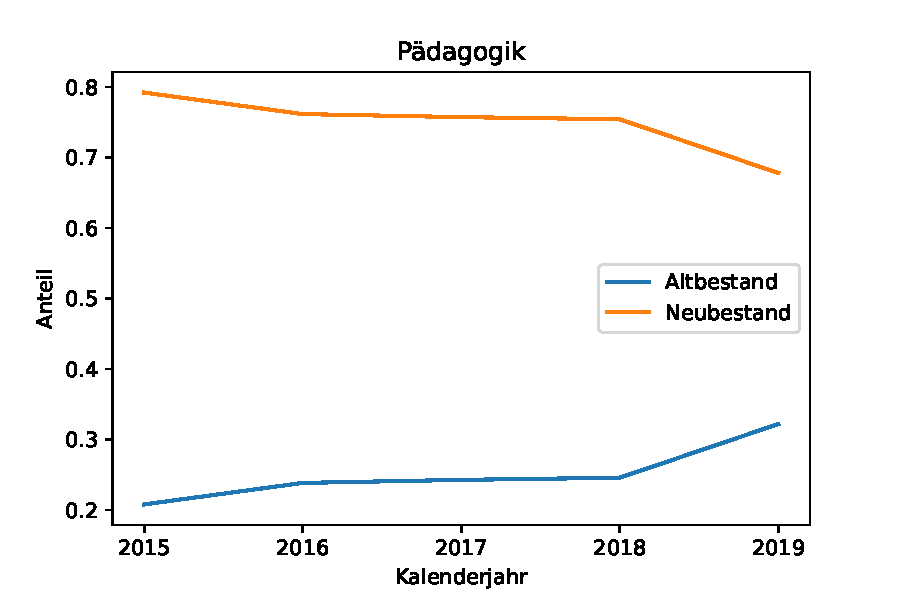
\includegraphics[width = 1\textwidth]{pad2.pdf}
        \end{subfigure}
        \begin{subfigure}{0.49\textwidth}
            
            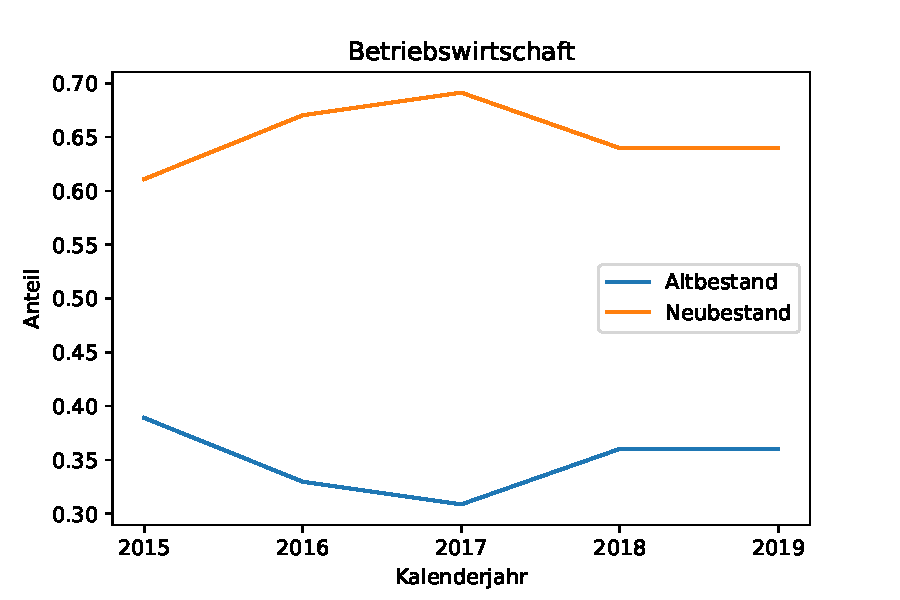
\includegraphics[width = 1\textwidth]{bwl2.pdf}
        \end{subfigure}
        \begin{subfigure}{0.49\textwidth}
           
            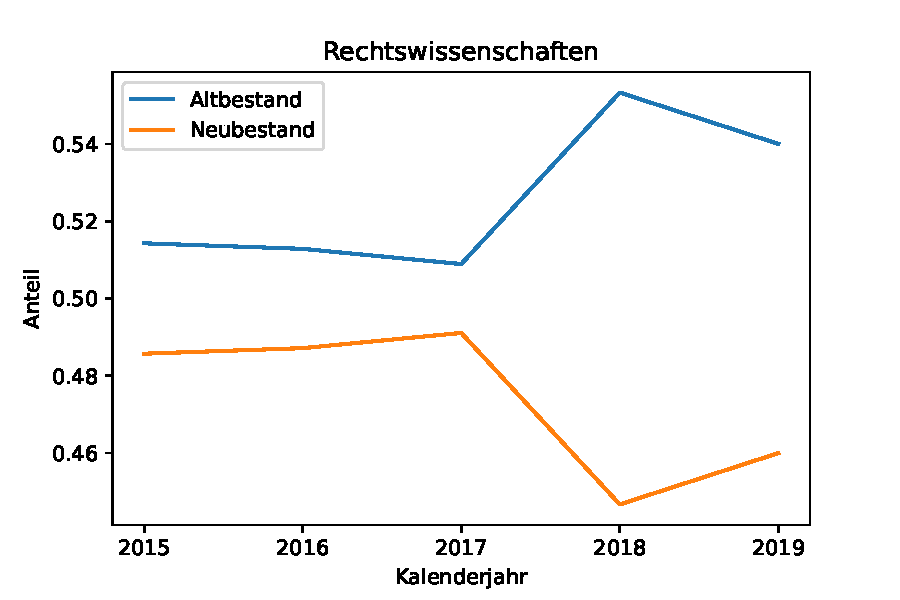
\includegraphics[width = 1\textwidth]{jus2.pdf}
        \end{subfigure}
        \begin{subfigure}{0.49\textwidth}
            
            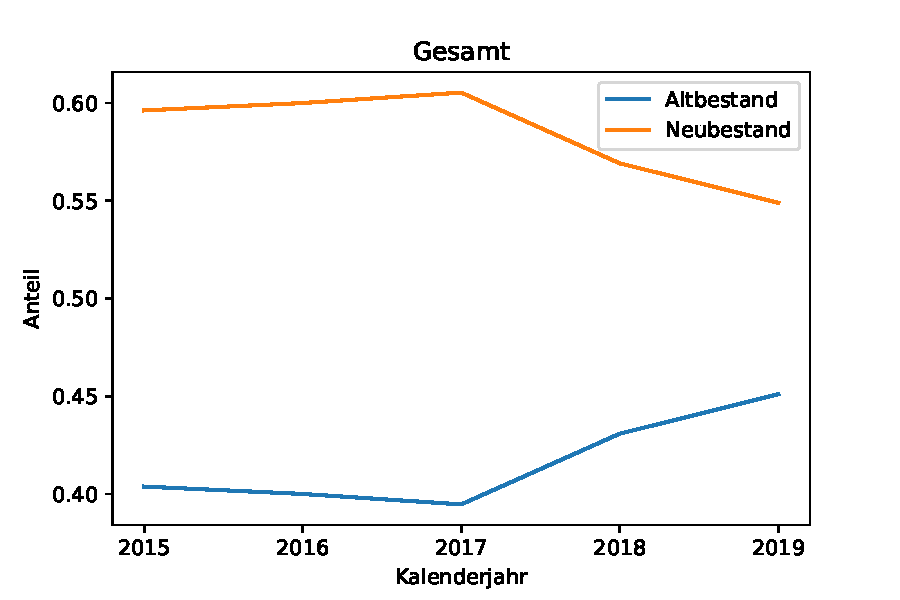
\includegraphics[width = 1\textwidth]{ges2.pdf}
        \end{subfigure}
            
    \end{figure}
    
\end{frame}

\begin{frame}
    Problem 1: \\
    Schätzung der prüfungsaktiven Studierenden, von denen bereits Anzahl und Merkmalskombinationen vorhanden sind \\[1cm]

    \pause

    Problem 2: \\
    Schätzung der prüfungsaktiven Studierenden, von denen weder Anzahl noch Merkmalskombinationen vorhanden sind    
\end{frame}

\begin{frame}{Herangehensweise Problem 1}
    \begin{itemize}
        \item Regression der ECTS \\[1cm]
        \pause
        \item Markov Ketten Modell \\[1cm]
        \pause
        \item Schätzung der Wahrscheinlichkeit aktiv zu sein, ohne zu klassifizieren
    \end{itemize}
    
\end{frame}

\begin{frame}{Ergebnisse für Ansatz 1 (P1)}
    \pause
    \scriptsize{
    \begin{table}[ht]
        \begin{tabular}{ p{1cm} p{1cm} p{1.5cm} p{1.5cm} p{1.5cm} p{1.5cm} }
          Metrik &               & lineare Regression & Random Forest  & SVM            & KNN \\
          \hline
          \multirow{2}{3em}{RMSE}
                 & 1 Jahr        & $18.7 \pm 0.2$     & $19.2 \pm 0.3$ & $19.7 \pm 0.4$ & $18.7 \pm 0.3$       \\
                 & $\geq$ 2 Jahre & $16.8 \pm 0.2$     & $15.4 \pm 0.2$ & $19.2 \pm 0.3$ & $14.8 \pm 0.2$        \\
      
          \hline
          \multirow{2}{3em}{MAE}
                 & 1 Jahr        & $15.6$             & $15.9$         & $15.9$         & $14.5$        \\
                 & $\geq$ 2 Jahre & $13.3$             & $11.7$         & $16.2$         & $10.4$        \\
      
          \hline
        \end{tabular}
      \end{table}
    }
    
\end{frame}

\begin{frame}{Ergebnisse für Ansatz 2 (P1)}
    \pause    
    \begin{scriptsize}
		\tikzfig{fig1}
	\end{scriptsize}
\end{frame}

\begin{frame}{Ergebnisse für Ansatz 2 (P1)}
    \footnotesize{
    $\left[ \begin{array}{rrrr}  0.05 & 0.19 & 0.53 & 0.23  \end{array}\right]$,
    $\left[ \begin{array}{rrrr} 0 & 0 & 0 & 0 \\  0 & 0 & 0 & 0 \\ 0.02 & 0.13 & 0.79 & 0.07 \\ 0.02 & 0.49 & 0.19 & 0.29 \end{array}\right]$,
    $\left[ \begin{array}{rrrr} 0 & 0 & 0 & 0 \\  0 & 0 & 0 & 0 \\ 0.01 & 0.05  & 0.82  & 0.13 \\ 0.01 & 0.46 & 0.24 & 0.29 \end{array}\right]$,
    $\left[ \begin{array}{rrrr} 0 & 0 & 0 & 0 \\  0 & 0 & 0 & 0 \\ 0.05 & 0.01 & 0.83 & 0.11\\ 0.00& 0.18 & 0.25 & 0.50\end{array}\right]$.
    }
\end{frame}



\begin{frame}{Ergebnisse für Ansatz 3 (P1)}
    \pause
    \scriptsize{
    \begin{table}[ht]
        \begin{tabular}{ p{1.5cm} p{1.5cm} p{1cm} p{1cm} p{1cm} p{1cm} }
                         &                  & log. Reg.                                  & RF                                         & SVM                                        & KNN                                        \\
          \hline
          \multirow{2}{3em}{1 Jahr}
                         & Predicted        & 129.39                                     & 128.17                                     & 128.84                                     & 129.29                                     \\
                         & Real             & 129                                        & 129                                        & 129                                        & 129                                        \\
      
          \multirow{2}{2.5cm}{$\geq$ 2 Jahre}
                         & Predicted        & 121.25                                     & 117.46                                     & 120.59                                     & 120.9                                      \\
                         & Real             & 121                                        & 121                                        & 121                                        & 121                                        \\
          \hline

        \end{tabular}
      \end{table}
    }
\end{frame}

\begin{frame}{Ergebnisse für Problem 1}
    \pause
    \small{
    \begin{itemize}
        \item[\textcolor{red}{X}] Ansatz 1 funktioniert nicht - zu große Fehler bei Schätzung der ECTS \pause
        \item[\textcolor{red}{X}] Ansatz 2 benötigt mehr Daten, um ihn seriös zu erproben \pause
        \item[\textcolor{green}{\checkmark}] Ansatz 3 funktioniert auf kleinem Datensatz (sehr!) gut - man benötigt mehr Daten um ihn noch besser zu erproben
    \end{itemize}
    }
    
\end{frame}

\begin{frame}{Herangehensweise Problem 2}
    \begin{itemize}
        \item Schätzung der Anzahl der Studierenden mit gleicher Merkmalskombination wie im Jahr zuvor \\[1cm]
        \pause
        \item Clustering der Studierenden und anschließende Schätzung der Anzahl nach Cluster
    \end{itemize}
    
\end{frame}

\begin{frame}{Ergebnisse für Problem 2}
    \scriptsize{
    \begin{table}[ht]
        \begin{tabular}{ p{1cm} p{1cm} p{2.5cm} p{2cm} }
          Zeitspanne der Sch\"atzung &   & Prediction dummy Daten (Anzahl gegeben) & tats\"achliche Anzahl \\
          \hline
          \multirow{2}{3em}{1 Jahr}
                                     & 2016                   & 1105                                    & 1092                  \\
                                     & 2017                   & 984                                     & 973                   \\
          \hline
          \multirow{2}{4em}{2 Jahre}
                                     & 2016                   & 878                                     & 819                   \\
                                     & 2017                   & 769                                     & 721                   \\
          \hline
        \end{tabular}
      \end{table}
    } \pause
    \small{
    \begin{itemize}
        \item[\textcolor{orange}{$\sim$}] Legitimation von Ansatz 1 für Problem 2 \pause
        \item[\textcolor{orange}{$\sim$}] Zu wenige Daten vorhanden, um Ansatz 2 für Problem 2 seriös zu erproben
    \end{itemize}
    }
\end{frame}

\begin{frame}{Beiträge}
    \pause
    Klare Darstellung der Problemstellung \\[1cm]
    \pause
    Erprobung unterschiedlicher Ansätze \\[1cm]
    \pause
    Machine Learning Ansatz für Problem 1, der gute Ergebnisse liefert \\[1cm]
    \pause
    Notwendigkeit von mehr Daten, um Ansätze weiter zu Erproben
    
\end{frame}




\end{document}